\documentclass{standalone}
\usepackage{tikz}
\usepackage{mathrsfs}
\usetikzlibrary{positioning, shapes.geometric, arrows}
\tikzstyle{startstop} = [draw, rectangle, rounded corners, minimum width=3cm, minimum height=1cm,text centered, draw=black]
\tikzstyle{bola} = [draw, circle , minimum size = 10, draw=black, text centered]
\tikzstyle{elipse} = [draw, ellipse, minimum height = 10]
\usepackage[T1]{fontenc}
\renewcommand*\familydefault{\ttdefault} %% Only if the base font of the document is to be typewriter style
\begin{document}
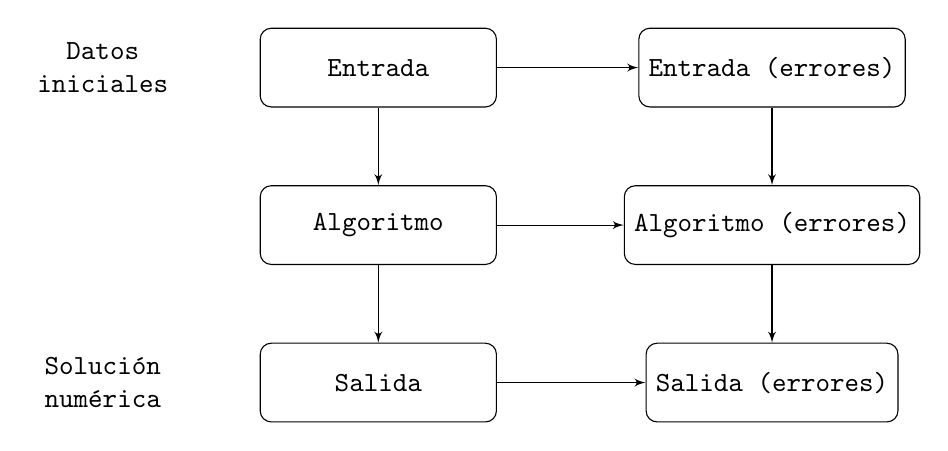
\begin{tikzpicture}[=>stealth, auto, node distance = 2cm, >=latex',every text node part/.style={align=center}]

\node (start1) [startstop] {Entrada};  
\node (start2) [startstop, below of = start1] {Algoritmo};  
\node (start3) [startstop, below of = start2] {Salida};  
\node (iniciales) [node distance = 3.5cm, left of = start1]{Datos \\ iniciales};
\node (solucion) [node distance = 3.5cm, left of = start3]{Soluci\'{o}n \\ num\'{e}rica};

\draw [->] (start1) -- (start2);  
\draw [->] (start2) -- (start3);  

\node (start4) [startstop, node distance = 5cm, right of = start1] {Entrada (errores)};  
\node (start5) [startstop, node distance = 5cm, right of = start2] {Algoritmo (errores)};  
\node (start6) [startstop, node distance = 5cm, right of = start3] {Salida (errores)};  

\draw [->] (start4) -- (start5);
\draw [->] (start5) -- (start6);  

\draw [->] (start1) -- (start4);
\draw [->] (start2) -- (start5);
\draw [->] (start3) -- (start6);
\end{tikzpicture}
\end{document}